\documentclass[11pt]{exam}
\usepackage{listings}
\usepackage{pdfsync}

%
%  Created by Brad Miller on 2005-05-13.
%  Copyright (c) 2005 Luther College. All rights reserved.
%
%

\usepackage{subfigure}
\usepackage[pdftex]{graphicx}


%
%  Update these values for running headers
%
\firstpageheader{\bf\Large CS-160}{\bf\Large Final Exam}{\bf\Large
  May 18, 2016 }
\runningheader{CS 160}{}{Final Exam}
\addpoints

\begin{document}

\begin{center}
  \fbox{\fbox{\parbox{5.5in}{\centering This Exam is being given under
        the guidelines of the \textbf{Honor Code}. You are expected to
        respect those guidelines and to report those who do not.
        Answer the questions in the spaces provided. If you run out of
        room for an answer, continue on the back of the page.  There are
      \numquestions\  questions for a total of  \numpoints\ points.}}}
\end{center}

% setup standard options for the including code fragments
\lstset{language=Python,numbers=left}

\vspace{0.1in}
\hbox to \textwidth{Name:\enspace\hrulefill}

% Questions start here:
\begin{questions}

\question[5] Which of the following algorithms and/or data structures could be used to implement the Map ADT (That is, a data structure that acts like a Python dictionary)?
\begin{itemize}
\item A List and the Binary Search algorithm.
\item A Heap
\item A Binary Search Tree
\item A Hash Table
\item A Stack
\end{itemize}

\question[2] Which of the above possibilities would be the best choice
\vspace{1in}

\question[3] What are the three laws of recursion?
\vspace{1in}

% \question[10]  Recall that the height of the tree is defined as the number of edges between the root and the deepest leaf in the tree.  Write a recursive function height(t) that takes a tree as a parameter and returns the height of the tree.  \textit{Hint 1:} The methods for a tree are as follows:
% \begin{itemize}

%     \item BinaryTree()  Create a new instance of a binary tree.
%     \item getLeftChild() Return the binary tree corresponding to the left child of the current node or None if no child.
%     \item getRightChild() Return the binary tree corresponding to the right child of the current node or None if no child.
%     \item setRootVal(x) Store the object in parameter x in the current node.
%     \item getRootVal() Return the object stored in the current node.
%     \item insertLeft(x) Create a new binary tree and install it as the left child of the current node.
%     \item insertRight(x) Create a new binary tree and install it as the right child of the current node.

% \end{itemize}

% \textit{Hint 2:} The height function is very simple (and short) if you think recursively

\question[10] Given the following list \lstinline{L = [1, 3, 5, 7, 9, 11, 13, 17, 19, 23]} write down each comparison that the \texttt{binarySearch} algorithm would do when searching for the key 7.
\vspace{4in}

\question[10]
A palindrome is a string that reads the same both forward and
backward. We can ignore punctuation marks and white space. Palindromes have been
 around since biblical times. For example, when Adam and Eve first met Adam is quoted as saying ``madam I'm adam''. Later in history a large engineering feat in central america was described as:
``a man a plan a canal panama''. When the use of electricty became widespread,
engineers were often heard muttering ``so many dynamos''.   More simply, ``abcba'' is a palindrome.  Write a recursive
function \texttt{pal(s)} to dermine whether a given string is a
palindrome. For example: \texttt{pal(palprep("radar"))}
would return true, whereas \texttt{pal("palindrome")} would return false. \textit{Hint: a zero or one character string is always a palindrome, a two character string is a palindrom if the two characters are the same... And, don't forget how to slice}

\newpage
\question Given the following list of numbers \lstinline{x = [13, 24, 5, 7, 9, 17, 32, 27, 2]}

\begin{parts}
\part[10]  Create a binary search tree and insert each of the numbers.  Draw a picture of the final tree.  You do not need to show all the intermediate trees, just the final.
\vspace{3in}

\part[10]  Create a binary min-heap and insert the numbers one at a time into the heap. Draw both the tree and list representation of the heap after all the numbers are inserted.
\vspace{3in}

\part[5] Show the new binary search tree after you have deleted the nodes 7, 24, and 13.
\vspace{3in}

\part[5] Show the new heap after you have called the delMin (dequeue) method 2 times.

\end{parts}

\newpage
\question[10] Given the following set of hash keys show the resulting hash table assuming that you are using linear probing.  Insert them in order from left to right.  The table holds exactly 11 keys.  You do not need to worry about growing the table.

\begin{table}[h!]
    \begin{center}
    \begin{tabular}{|c|c|c|c|c|c|c|c|c|}
    113 & 117 & 97 & 100 & 114 & 108 & 116 & 105 & 99 \\
     \end{tabular}
     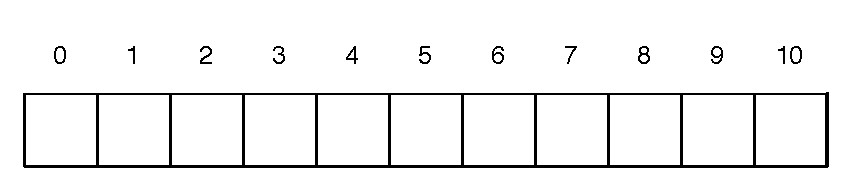
\includegraphics{hash_table_11}
    \end{center}
    \label{htab}
\end{table}


\question[10] Given the following list \lstinline{L = [90, 1, 3, 8, 56]}.  Show the contents of \lstinline{L} after each pass of Insertion sort.  I'll give you pass 1 for free!
\begin{center}
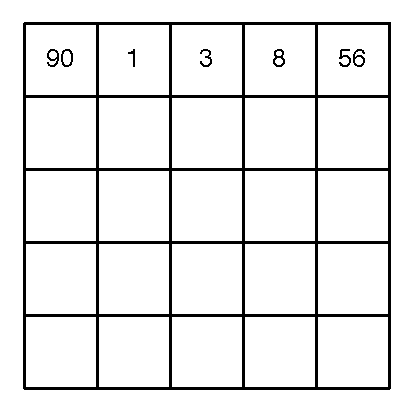
\includegraphics{insertion_boxes}
\end{center}

\question[10] Given the following list
\lstinline{L = [11, 3, 23, 17, 9, 21, 7, 5, 1, 19, 13, 15]}.  Show the contents of \lstinline{L} after one partition by \texttt{Quicksort}.  You should use the median of three pivot selection method.
\vspace{4.5in}

% \question[10] Given the following list \lstinline{L = [90, 1, 3, 8, 56, 21, 5, 13, 1, 146, 2, 34]}.  Show the contents of \lstinline{L} after the After all the swapping is done for a gap size of 3 using Shell sort.
%
% \begin{center}
% 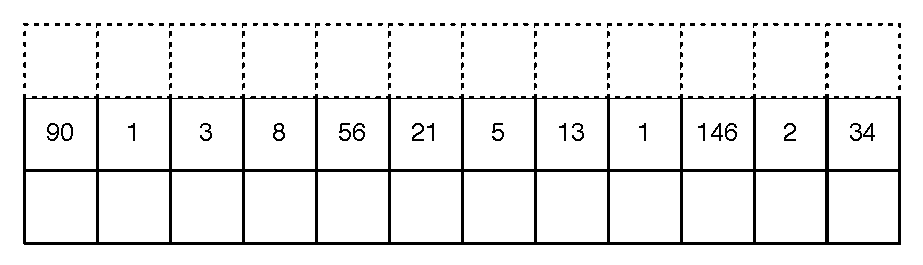
\includegraphics{shell_gaps}
% \end{center}

\newpage
\question Given the binary tree shown below:
\begin{figure}[h!]
    \begin{center}
        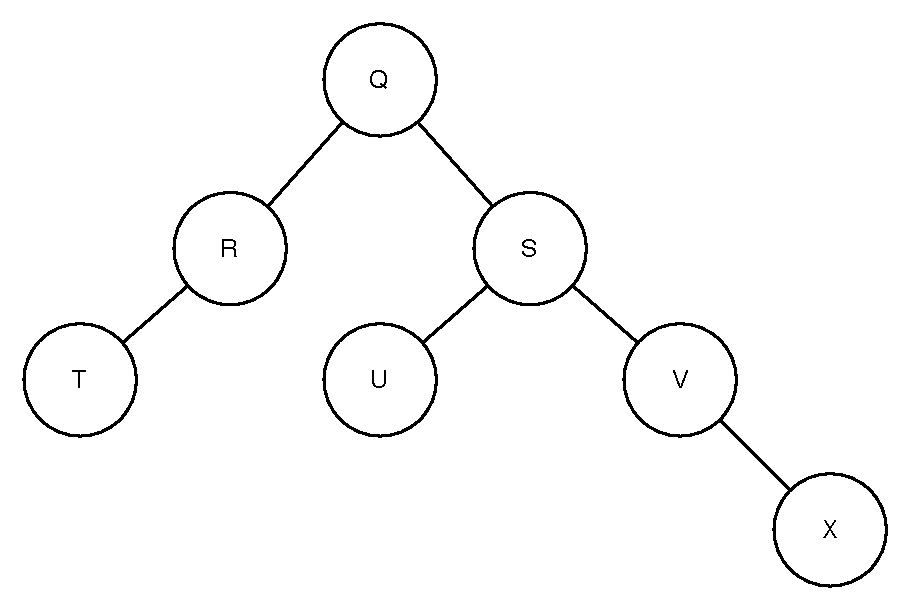
\includegraphics[height=3in]{binaryTree}
    \end{center}
\end{figure}
\begin{parts}
    \part[5] Perform a pre-order traversal of the tree.  Write out the name of each node in the order it is visited.
    \vspace{1in}
    \part[5] Perform a post-order traversal of the tree. Write out the name of each node in the order it is visited.
    \vspace{1in}
    \part[5] Draw the list of lists representation for the tree rooted at node ``s''.
\end{parts}

\newpage

\newpage

% \newpage
\question[10] Given the following directed graph, draw the adjacency matrix representation of the graph.  You can assume that the weights for all the links are 1.
\begin{figure}[h!t]
        \begin{center}
        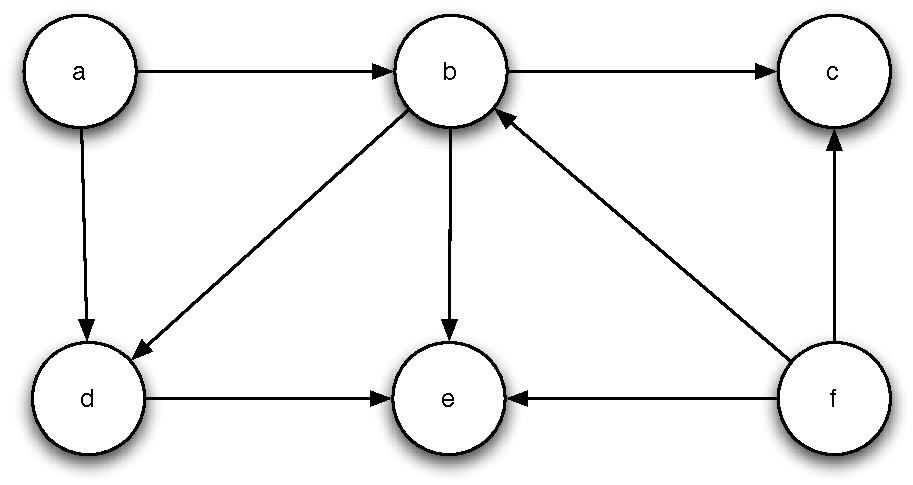
\includegraphics[scale=.75]{dfs}
    \end{center}
\end{figure}


\question[10] Perform a depth first search on the graph starting using node a as the starting vertex.  Draw the predecessor links, and add the distance values to the graph.

\end{questions}


\end{document}
